\documentclass[a4paper, 11pt, titlepage]{article}
\usepackage[utf8]{inputenc}
\usepackage[czech]{babel}
\usepackage[total={18.5cm,25cm}, top=3cm, left=1.25cm, includefoot]{geometry}
\usepackage{fancyhdr}
\usepackage{amsmath} % větší zlomyk pmocí \dfrac
\usepackage{graphicx}
\usepackage{float} % H aby neuplavali
\usepackage{ctable} % horozontální čára s nastavitelnou šířkou a mezerami od okolí \specialrule{1pt}{0pt}{0pt} 
\usepackage{array}
\usepackage{caption}
\usepackage{subcaption}

\newcommand{\nazevprace}{PROTOKOL O MĚŘENÍ}
\newcommand{\uloha}{ZESILOVAČ - OSCILÁTOR}
\newcommand{\pcislo}{101-4R} 			% číslo protokolu

\newcommand{\trida}{4A}
\newcommand{\skupina}{3}
\newcommand{\jmeno}{Jan}
\newcommand{\prijmeni}{VYKYDAL}
\newcommand{\porc}{26}						% pořadové číslo v třídní knize

\newcommand{\rok}{2014/2015}
\newcommand{\datm}{14.1.} 				% datum měření
\newcommand{\dato}{21.1.} 				% datum odevzdání


\pagestyle{fancy}
\fancyhf{}

\fancyfoot[C]{
  \begin{tabular}[H]{|c|c|c|c|}
    \hline
    \textbf{Jméno PŘÍJMENÍ:} \jmeno~\prijmeni & \textbf{Třída:} \trida & \textbf{Číslo protokolu:} \pcislo & \textbf{List:} \thepage/\pageref{konec} \\
    \hline
  \end{tabular}
}

\renewcommand{\headrulewidth}{0.0pt}
%\renewcommand{\footrulewidth}{0.4pt}


\begin{document} 
	
	
	\renewcommand{\figurename}{Schéma č.}
	\renewcommand{\tablename}{Tabulka č.}
	
  \begin{titlepage}
  \renewcommand{\arraystretch}{1.3}
  \pagestyle{empty}
  \begin{center}
    \begin{tabularx}{\textwidth}{!{\vrule width 2pt}XX!{\vrule width 1pt}XX!{\vrule width 1pt}XX!{\vrule width 1pt}X!{\vrule width 1pt}X!{\vrule width 1pt}X!{\vrule width 1pt}X!{\vrule width 2pt}}
      \specialrule{2pt}{0pt}{0pt}
      \multicolumn{10}{!{\vrule width 2pt}c!{\vrule width 2pt}}{\Large Vyšší odborná škola a Střední průmyslová škola elektrotechnická} \\
      \multicolumn{10}{!{\vrule width 2pt}c!{\vrule width 2pt}}{\Large Božetěchova 3, Olomouc} \\
      \multicolumn{10}{!{\vrule width 2pt}c!{\vrule width 2pt}}{\Large Laboratoře elektronických měření} \\
      \specialrule{1pt}{0pt}{0pt} 
      \multicolumn{10}{!{\vrule width 2pt}c!{\vrule width 2pt}}{} \\
      \multicolumn{10}{!{\vrule width 2pt}c!{\vrule width 2pt}}{\bf\Huge \nazevprace} \\
      \multicolumn{10}{!{\vrule width 2pt}c!{\vrule width 2pt}}{} \\
      \specialrule{1pt}{0pt}{0pt}
      
      
      \multicolumn{8}{!{\vrule width 2pt}l!{\vrule width 1pt}}{Název úlohy} &
      \multicolumn{2}{l!{\vrule width 2pt}}{Číslo úlohy} \\
      \multicolumn{8}{!{\vrule width 2pt}c!{\vrule width 1pt}}{
      %	\begin{minipage}[H][16mm][c]{12cm}
      %		\begin{center}	
      			\Large\bf \uloha
      %		\end{center}
      %	\end{minipage}	
      } &
      \multicolumn{2}{c!{\vrule width 2pt}}{\Large\bf \pcislo} \\
      \specialrule{1pt}{0pt}{0pt} 
      
      \multicolumn{10}{!{\vrule width 2pt}l!{\vrule width 2pt}}{Zadání} \\
      \multicolumn{10}{!{\vrule width 2pt}c!{\vrule width 2pt}}{\begin{minipage}[H][11.48cm][c]{0.8\textwidth}
  \begin{enumerate}
    \item
      Ověřte měřením některé katalogové údaje OZ MAA 741
      	\begin{enumerate}
      		\item
      			Napěťová nesymetrie OZ
      		\item
      			Rychlost přeběhu OZ
      	\end{enumerate}
    \item
      Podle zadání vyučujícího sestavte a realizujte OZ jako stejnosměrný meinvertující zesilovač se zatěžovacím rezistorem $R_L = 10~k\Omega$. Měřením ověřte zadanou hodnotu~$A_u$.
    \item
			U navrřeného zesilovače změřte horní mezní frekvenci, nakreslete na mm papír frekvenční přenosovou charakteristiku.
		\item
			Změřte a zekreslete závislost $f_H = f(A_u)$
	\end{enumerate}
\end{minipage}


} \\      
      \specialrule{1pt}{0pt}{0pt} 
      
      \multicolumn{1}{!{\vrule width 2pt}l!{\vrule width 1pt}}{Poř. č.} &
      \multicolumn{5}{l!{\vrule width 1pt}}{PŘÍJMENÍ a Jméno} &
      \multicolumn{1}{c!{\vrule width 1pt}}{Třída} &
      \multicolumn{1}{c!{\vrule width 1pt}}{Skupina} &
      \multicolumn{2}{l!{\vrule width 2pt}}{Školní rok} \\
      \specialrule{1pt}{0pt}{0pt} 
      
      \multicolumn{1}{!{\vrule width 2pt}c!{\vrule width 1pt}}{\Large\bf \porc} &
      \multicolumn{5}{c!{\vrule width 1pt}}{\Large\bf\prijmeni~\jmeno} &
      \multicolumn{1}{c!{\vrule width 1pt}}{\Large\bf \trida} &
      \multicolumn{1}{c!{\vrule width 1pt}}{\Large\bf \skupina} &
      \multicolumn{2}{c!{\vrule width 2pt}}{\Large\bf \rok} \\
      \specialrule{1pt}{0pt}{0pt} 
      
      \multicolumn{2}{!{\vrule width 2pt}l!{\vrule width 1pt}}{Datum měření} &
      \multicolumn{2}{l!{\vrule width 1pt}}{Datum odevzdání} &
      \multicolumn{2}{l!{\vrule width 1pt}}{Počet listů} &
      \multicolumn{4}{c!{\vrule width 2pt}}{Klasifikace} \\
      \specialrule{1pt}{0pt}{0pt} 
          
      \multicolumn{2}{!{\vrule width 2pt}c!{\vrule width 1pt}}{} &
      \multicolumn{2}{c!{\vrule width 1pt}}{} &
      \multicolumn{2}{c!{\vrule width 1pt}}{} &
      
      \multicolumn{1}{c!{\vrule width 1pt}}{příprava} &     
      \multicolumn{1}{c!{\vrule width 1pt}}{meření} &     
      \multicolumn{1}{c!{\vrule width 1pt}}{protokol} &     
      \multicolumn{1}{c!{\vrule width 2pt}}{obhajoba} \\
      
      
      \multicolumn{2}{!{\vrule width 2pt}c!{\vrule width 1pt}}{\Large\bf \datm} &
      \multicolumn{2}{c!{\vrule width 1pt}}{\Large\bf \dato} &
      \multicolumn{2}{c!{\vrule width 1pt}}{\Large\bf \pageref{konec}} &
      \multicolumn{1}{c!{\vrule width 1pt}}{} &     
      \multicolumn{1}{c!{\vrule width 1pt}}{} &     
      \multicolumn{1}{c!{\vrule width 1pt}}{} &     
      \multicolumn{1}{c!{\vrule width 2pt}}{} \\     
      &&&&&&&&&\\
      \specialrule{1pt}{0pt}{0pt} 
       
      \multicolumn{10}{!{\vrule width 2pt}X!{\vrule width 2pt}}{\begin{tabular}{lll}
  \hspace*{2.5cm} & Teoretický úvod             & Tabulky naměřených a vypočtených hodnot \\
  \hspace*{2.5cm} & Schéma                      & Vzor výpočtu                            \\
  \hspace*{2.5cm} & Tabulka použitých přístrojů & Grafy                                   \\
  \hspace*{2.5cm} & Postup měření               & Závěr                                   \\
\end{tabular}
} \\
      \specialrule{2pt}{0pt}{0pt} 
    \end{tabularx}  
  \end{center}
\end{titlepage}

  \setcounter{page}{2}
  \section{Teoretický úvod}
  \indent\indent
 Slovo dioda je uměle vytvořené slovo z řeckého slova ,,di'' (dva) a koncovky slova elektroda. Polovodičová dioda má obvykle dva vývody nazývané anoda a katoda, anoda je připojena k části polovodičového krystalu označovaného P (Positive) a katoda k části polovodičového krystalu označovaného N (Negative). Diody de vyrábí dopováním polovodiče, tj. přidáváním příměsí do polovodiče. Jako příměsi se používají prvky které mají o jeden valenční elektron více pro vytvoření krystalu N, tyto prvky se nazývají donory, nebo prvky které mají o jeden valenční elektron méně, pro vytváření krystalů P, tyto prvky se nazývají akceptory.
  
  \subsection{výroba PN přechodu}
  	\indent\indent
  	Přechod se vyrábí jak již bylo zmíněno dotování polovodičové destičky příměsemi. Na polovodičovou destičku se položí nečistota která je tvořena atomy co mají ve valenční vrstvě o jeden elektron méně než polovodičová destička. Na druhou část destičky se položí nečistota která je tvořena elektrony, které mají ve valenční vrstvě o jeden elektron více než polovodičová destička. Tato destička se zahřeje v peci na teplotu přibližně~$600~^\circ C$.
  	
  	Po zatavení nečistot do polovodiče dojde k rekombinaci elektronů a děr na rozhraní přechodů PN. Po určitém čase bude vlivem rekombinace vytvořena zóna v oblasti přechodu PN, takřka bez volných nosičů náboje. Tento přechod bývá označován jako hradlová vrstva. Po vytvoření této hradlové vrstvi již k další rekombinaci nedochází. I přesto že mezi přechody PN hradlová vrstva je, dochází vlivem okolní teploty k velmi malému proudu elektronů přechodem PN. 
  
  \subsection{PN v propustném směru}
  	\indent\indent
  	Připojíme-li anodu na kladný pól zdroje a katodu na záporný pól zdroje, a napětí zdroje bude dostatečné k překonání hradlové vrstvy, toto napětí bývá označované jako prahové napětí, začne přechodem PN procházet proud.
  	
  \subsection{PN v závěrném směru}
  	\indent\indent
  	Připojíme li k anodě záporný pól zdroje a ke katodě kladný pól zdroje, dojde k přitažení volných elektronů ke katodě a pohybu děr k anodě, důsledkem této události dojde k rozšíření hradlové vrstvy. Tohoto jevu se používá u varikapů.

	\subsection{Zatěžovací přímka}
		\indent\indent
		Zatěžovací přímka slouží ke graficko-početní metodě analýzy obvodů s lineárním a nelineárním prvkem. V průsečíku zatěžovací přímky a VACH nelineárního prvku sestrojíme kolmice k osám x, y a odečteme z osy x napětí na nelineárním prvku a z osy y proud v obvodu.
		
		Úsekový tvar přímky:
		\begin{equation}
  		\dfrac{x}{p} + \dfrac{y}{q} = 1
  	\end{equation}
		
		\hspace*{2cm}kde:\newline    
  	\hspace*{4cm}$x$ \dotfill souřadnice x bodu náležícího této přímce\hspace*{4cm}\newline
  	\hspace*{4cm}$y$ \dotfill souřadnice y bodu náležícího této přímce\hspace*{4cm}\newline
  	\hspace*{4cm}$p$ \dotfill souřadnice x bodu ležícího na ose x\hspace*{4cm}\newline
  	\hspace*{4cm}$q$ \dotfill souřadnice y bodu ležícího na ose y\hspace*{4cm}\newline

		
		Odvození rovnice pro zatěžovací přímku:
		\begin{eqnarray}
      U_D + U_R &=& U \nonumber\\
      U_D + IR &=& U \nonumber\\
      \dfrac{U_D}{U} + \dfrac{IR}{U} &=& 1
    \end{eqnarray}
		  
		\hspace*{2cm}kde:\newline    
		\hspace*{4cm}$U$ \dotfill suma všech úbytků napětí v obvodu\hspace*{4cm}\newline
		\hspace*{4cm}$U_D$ \dotfill úbytek napětí na diodě\hspace*{4cm}\newline
		\hspace*{4cm}$I$ \dotfill proud protékající obvodem\hspace*{4cm}\newline
		\hspace*{4cm}$R$ \dotfill předřadný rezistor\hspace*{4cm}\newline		
  	
  	Odvození bodů zatěžovací přímky:
  	\begin{eqnarray}
      \dfrac{U_D}{U} + \dfrac{0}{U} &=& 1 \nonumber\\
      U_D &=& = U \nonumber\\
      P &=& [U; 0] \\      
      \dfrac{0}{U} + \dfrac{IR}{U} &=& 1 \nonumber\\
      I &=& \dfrac{U}{I} \nonumber\\
      Q &=& \left[0; \dfrac{U}{R}\right]
    \end{eqnarray}
    		  
		\hspace*{2cm}kde:\newline    
		\hspace*{4cm}$U$ \dotfill suma všech úbytků napětí v obvodu\hspace*{4cm}\newline
		\hspace*{4cm}$U_D$ \dotfill úbytek napětí na diodě\hspace*{4cm}\newline
		\hspace*{4cm}$I$ \dotfill proud protékající obvodem\hspace*{4cm}\newline
		\hspace*{4cm}$R$ \dotfill předřadný rezistor\hspace*{4cm}\newline		
		\hspace*{4cm}$P$ \dotfill souřadnice bodu ležícího na ose x\hspace*{4cm}\newline
  	\hspace*{4cm}$Q$ \dotfill souřadnice bodu ležícího na ose y\hspace*{4cm}\newline
  	
  \subsection{Dynamický (diferenciální) odpor}
  	\indent\indent
  	Pokud pracujeme se součástkou který má nelineární VACH, tak si výpočty můžeme zjednodušit tak, že v jednom konkrétním pracovním bodě si spočítáme diferenciální odpor, pomocí tohoto diferenciálního odporu můžeme počítat s nelineárním prvkem v konkrétním pracovním bodu, jakoby byl lineární.
  	
  	\subsubsection{Graficko-početní metoda zjištění diferenciálního odporu}
  		\indent\indent
  		Na VACH si zvolíme konkrétní pracovní bod, k tomuto pracovnímu bodu sestrojíme tečnu. V libovolném místě k tečně doplníme dvě strany a sestrojíme pravoúhlí trojúhelník, přičemž strana splývající s tečnou bude přepona, viz. graf č. 2.
  		
  		Výpočet diferenciálního odporu:  		
  		\begin{equation}
  			r_d = \dfrac{\Delta U}{\Delta I}
  		\end{equation}
  		
  		\hspace*{2cm}kde:\newline    
			\hspace*{4cm}$r_d$ \dotfill diferenciální odpor\hspace*{4cm}\newline
			\hspace*{4cm}$\Delta U$ \dotfill odvěsna pravoúhlého trojúhelníku rovnoběžná s osou x\hspace*{4cm}\newline
			\hspace*{4cm}$\Delta I$ \dotfill odvěsna pravoúhlého trojúhelníku rovnoběžná s osou y\hspace*{4cm}\newline
		
 

  \clearpage
  \section*{Schémata}
  \begin{figure}[H]
    \centering
    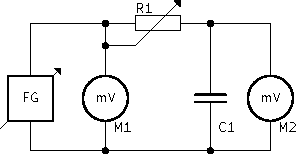
\includegraphics[width=7.5057cm]{../img/RC_au.pdf}
    \caption{Měření napěťového přenosu integračního článku}
    \label{sch:1}
  \end{figure}
  
  \begin{figure}[H]
    \centering
    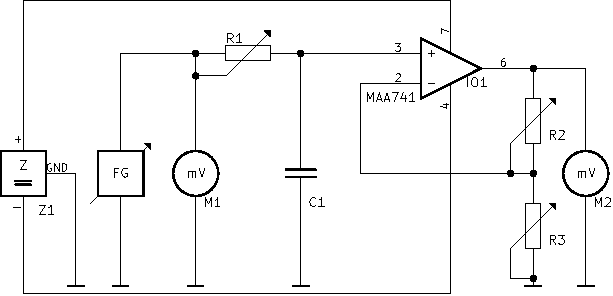
\includegraphics[width=15.5448cm]{../img/RC_OZ_au.pdf}
    \caption{Měření napěťového přenosu celého filtru}
    \label{sch:2}
  \end{figure}
  
  \begin{figure}[H]
    \centering
    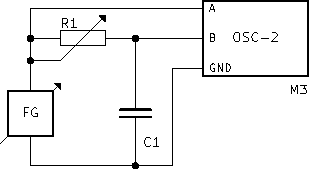
\includegraphics[width=7.8486cm]{../img/RC_phi.pdf}
    \caption{Měření fázového posunu mezi vstupním a výstupním napětím integračního článku}
    \label{sch:3}
  \end{figure}
  
  \begin{figure}[H]
    \centering
    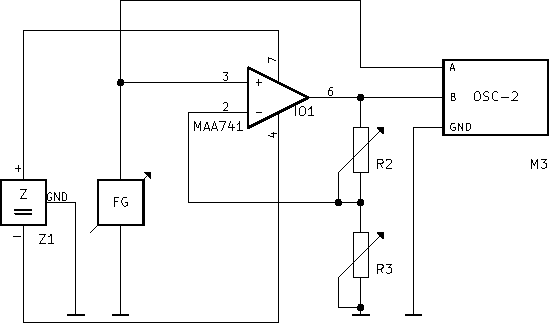
\includegraphics[width=13.9446cm]{../img/OZ_phi.pdf}
    \caption{Měření fázového posunu mezi vstupním a výstupním napětím operačního zesilovače}
    \label{sch:4}
  \end{figure}
  
  \begin{figure}[H]
    \centering
    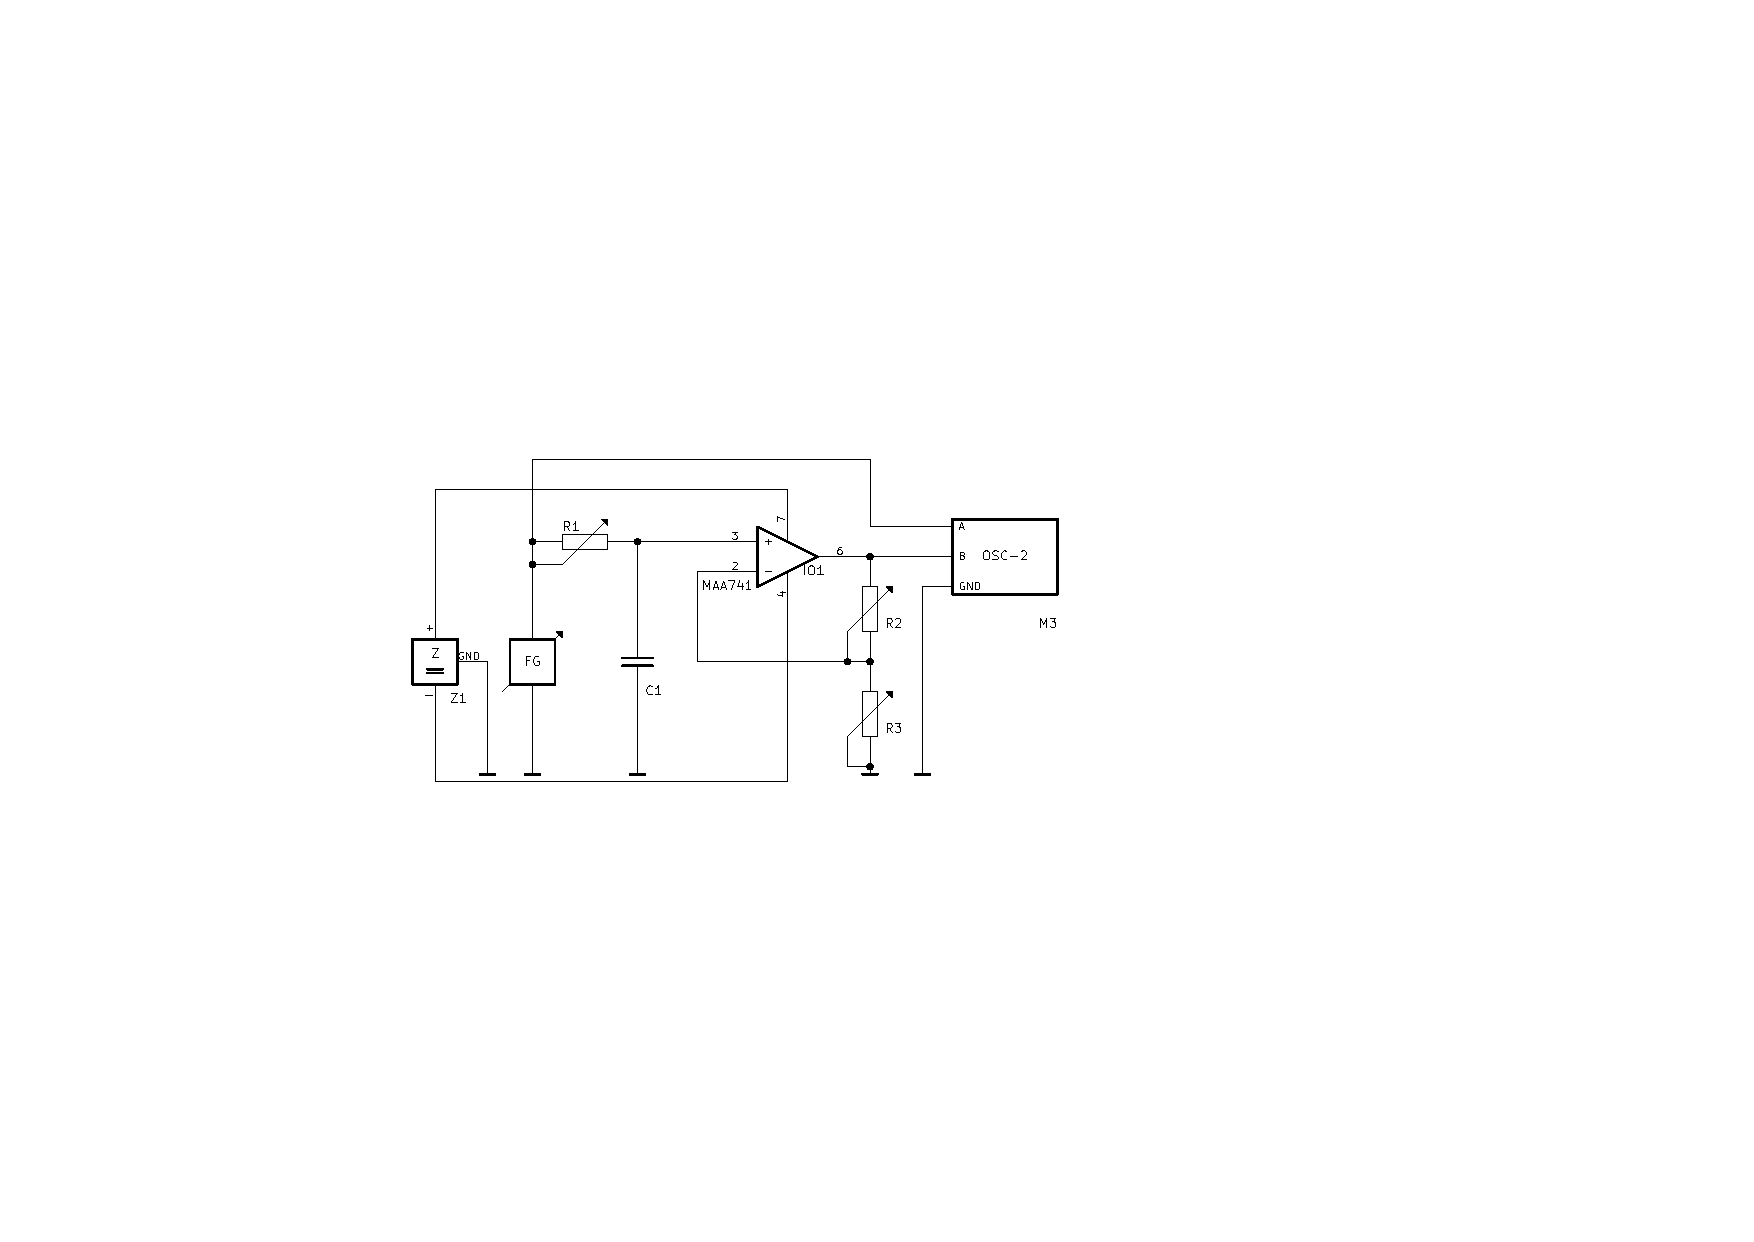
\includegraphics[width=16.4211cm]{../img/RC_OZ_phi.pdf}
    \caption{Měření fázového posunu mezi vstupním a výstupním napětím celého filtru}
    \label{sch:5}
  \end{figure}
  


  \section{Tabulka použitých přístrojů}
  \begin{table}[H]
    \begin{center}
      \begin{tabular}[H]{!{\vrule width 1pt}c|c|c|c|c!{\vrule width 1pt}}
      \specialrule{1pt}{0pt}{0pt} 
      \textbf{Označení v zapojení} & \textbf{Přístroj} & \textbf{Typ} & \textbf{Evidenční číslo} &\textbf{Poznámka} \\\specialrule{1pt}{0pt}{0pt} 
      
      $-$   & DMM           & MASTECH MY-64     & $0659$  & $-$ \\\hline
      $FG$  & generátor     & GoldStar FG-2002C & $0382$  & $-$ \\\hline
      $mV$  & milivoltmetr  & TESLA BK-128      & $0132$  & $-$ \\\specialrule{1pt}{0pt}{0pt} 
          
    \end{tabular}
      
      \caption{Tabulka použitých přístrojů}
      \label{tab:metr}      
    \end{center}
  \end{table}

  \section*{Postup měření}
  \subsection*{Zapojení obvodu}
    \begin{itemize}
      \item
      	Ze zadaných parametrů dopočítáme požadované hodnoty součástek.
      \item
      	Součástky, které jsme vypočítali připojíme k měřícímu přípravku.
      \item
        K obvodu připojíme měřící systém UNIMA a zdroj napětí. 	
	\end{itemize}

		
 

  \section*{Tabulky naměřených a vypočítaných hodnot} 
  
  \begin{table}[H]
    \begin{center}
      \begin{tabular}[H]{!{\vrule width 1pt}c|c|c|c|c|c|c|c!{\vrule width 1pt}}
        \specialrule{1pt}{0pt}{0pt} 
        č. m.	&	$f~[Hz]$	&	$U_{2_{RC}}~[V]$	&	$\delta_{\%U_{2_{RC}}}$	& $a_{U_{RC}}~[dB]$ &	$U_{2_{RCOZ}}~[V]$	&	$\delta_{\%U_{2_{RCOZ}}}$	& $a_{U_{RCOZ}}~[dB]$		\\\specialrule{1pt}{0pt}{0pt}
		1	&	100		&	1,00	&	4,000	&	0,000	&	3,00	&	4,000	&	9,542	\\\hline
		2	&	800		&	0,88	&	4,545	&	-1,110	&	2,60	&	4,615	&	8,299	\\\hline
		3	&	900		&	0,84	&	4,762	&	-1,514	&	2,50	&	4,800	&	7,959	\\\hline
		4	&	1000	&	0,82	&	4,878	&	-1,724	&	2,40	&	5,000	&	7,604	\\\hline
		5	&	1100	&	0,80	&	5,000	&	-1,938	&	2,30	&	5,217	&	7,235	\\\hline
		6	&	1200	&	0,76	&	5,263	&	-2,384	&	2,20	&	5,455	&	6,848	\\\hline
		7	&	1500	&	0,68	&	5,882	&	-3,350	&	2,00	&	6,000	&	6,021	\\\hline
		8	&	1800	&	0,61	&	6,557	&	-4,293	&	1,80	&	6,667	&	5,105	\\\hline
		9	&	40000	&	0,04	&	10,000	&	-27,959	&	0,10	&	4,000	&	-20,000	\\\hline
		10	&	100000	&	0,01	&	4,000	&	-40,000	&	0,04	&	10,000	&	-27,959
		
		\\\specialrule{1pt}{0pt}{0pt} 
        
      \end{tabular}
      
      \caption{napěťové přenosy $a_U$ integračního článku (index $RC$) a celého filtru (index $RCOZ$) měřeno při $U_1=1~V_{RMS}$}
      \label{tab:s1}      
    \end{center}
  \end{table}
 
 
  \begin{table}[H]
    \begin{center}
      \begin{tabular}[H]{!{\vrule width 1pt}c|c|c|c|c!{\vrule width 1pt}}
        \specialrule{1pt}{0pt}{0pt} 
        měřený obvod	&	$Y_1$	&	$Y_2$	& $sin(\varphi)$	&	$\varphi$	\\\specialrule{1pt}{0pt}{0pt} 
       	RC		&	14	&	10	&	0,714	&	$45^\circ 35^\prime 5 ^{\prime \prime}$	\\\hline
		OZ		&	11	&	1	&	0,091	&	$5^\circ 12^\prime 57 ^{\prime \prime}$	\\\hline
		RCOZ	&	8	&	6	&	0,750	&	$48^\circ 35^\prime 25 ^{\prime \prime}$

		\\\specialrule{1pt}{0pt}{0pt} 
        
      \end{tabular}
      
      \caption{fázové posuny získané pomocí metody Lissajousových obrazců, $Y_1$ znamená počet dílků od 0 do 1 na ose y, $Y_2$ znamená počet dílků od 0 do průsečíku osy y se zobrazovaným obrazcem}
      \label{tab:s1}      
    \end{center}
  \end{table}
  \section*{Vzory výpočtů}
  
  Výpočet geometrického průměru kondenzátoru $C$:
  \begin{equation}
    C = \sqrt{C_1 \cdot C_2} = \sqrt{34,16 \cdot 32,1} \doteq \underline{\underline{33,09~nF}}
    \nonumber
  \end{equation}
  
  Výpočet odporu rezistoru $R_1$ a $R_2$ provádíme dosazením do upraveného vztahu (1) pro dolní frekvenci 
  \begin{equation}
    R = \dfrac{1}{2\pi f_0 C} = \dfrac{1}{2\pi \cdot 300 \cdot 33,09 \cdot 10^{-9}} \doteq \underline{\underline{16~k\Omega}}
    \nonumber
  \end{equation}   
  
  Výpočet odporu rezistoru $R_1$ a $R_2$ provádíme dosazením do upraveného vztahu (1) pro horní frekvenci 
  \begin{equation}
    R = \dfrac{1}{2\pi f_0 C} = \dfrac{1}{2\pi \cdot 7000 \cdot 33,09 \cdot 10^{-9}} \doteq \underline{\underline{689~\Omega}}
    \nonumber
  \end{equation}     
  
  Střední hodnota výstupního napětí $U_{OUT_{AV}}$:
  \begin{equation}
    U_{OUT_{AV}} = \dfrac{U_{OUT_{MAX}} - U_{OUT_{MIN}}}{2} = \dfrac{7,4 - 7,3}{2}  \underline{\underline{7,35~V}}
    \nonumber
  \end{equation} 
    
  Výpočet procentní chyba výstupního napětí:
  \begin{equation}
    \delta_f = \dfrac{U_{OUT_{MAX}} - U_{OUT_MIN}}{U_{OUT_{AV}}} \cdot 100 = \dfrac{7,4 - 7,3}{7,35} \cdot 100 \doteq \underline{\underline{1,36~\%}}
  	\nonumber
  \end{equation}
  
  \section*{Grafy}


 
 
  \clearpage  
  \section{Závěr}
  
%  \begin{tabular}[H]{rcrl}
%    $20~V$ & $\pm0,5\%$ z MH $\pm 1$ digit & $19.99~V$ & $0,01~V$ \\
%    $2~mA$ & $\pm0,8\%$ z MH $\pm 1$ digit & $1.999~V$ & $0,001~mA$ \\
%    $20~mA$ & $\pm0,8\%$ z MH $\pm 1$ digit & $19.99~V$ & $0,01~mA$ \\
%    $200~mA$ & $\pm1,5\%$ z MH $\pm 5$ digit & $199.9~V$ & $0,1~mA$
%  \end{tabular}
  
  \subsection{Chyby měřících přístrojů}
    \indent\indent
    Procentuální chyba použitých DMM MASTECH-MY64 se pobybovala v intervalu $\pm0,714~\%$ až $\pm 6,5~\%>$. Přičemž nejmenší procentuální chyby byly na rozsahu $20~V$ a největší chyby byli na rozsahu $200~mA$. Naměřeným hodnotám bych ale nedával moc velkou váhu, protože na všech DMM blikala signalizace vybité baterie.
  
  \subsection{Zhodnocení}
    \begin{enumerate}
      \item
        V uvodu jsem shrnul základní poznatky o Zenerovích a lavinových diodách. Přižemž jsem se snažil zaměřit na jejich rozdíly a principy funkce.
      \item
        Vytvořil jsem graf VACH s využitím vlastního scriptu v pythonu využívajícího knihovnu pylab. Do grafu jsem vyznačil hodnoty I$_{ZD_{MIN}}$, U$_{ZD_{MIN}}$ a U$_{ZD_{MAX}}$. I$_{ZD_{MAX}}$ nebylo vyznačeno, protože v zadání bylo jen několik bodů na VA charakteristice. I$_{ZD_{MAX}}$ se ale nachází až za hranicí kterou sme měli měřit.
      \item
        Nakreslil jsem schéma zapojení paralerního stabilizátoru se Zenerovou diodou a vyznačil hlavní veličiny.
      \item
        Navrhnul jsem velikost rezistoru R$_1$ a to jak výpočtem tak experimentálně pomocí snížování hodnoty reostaru. Druhou jmenovanou metodou jsem došel k hodnotě $84~\Omega$. Pomocí mého orientačního výpočtu jsem dočelk k hodnotě $85,7~\Omega$, tato hodnota se sice od naměřené hodnoty liší o $1,7~\Omega$, ale jako odhad je to velmi dobrý výsledek.
      \item
        Sestavil jsem stabilizátor dle zadání a změril jsem:
        \begin{enumerate}
          \item
            V zadaném režimu obvod stabilizuje výstupní napětí.    
          \item            
            Změnou výstupního proudu $\Delta$I$_2 = 10~mA$ se výstupní napětí změní o $\Delta$U$_{ZD}~=~0,36~V$.
          \item
            Změnou vstupního napětí $\Delta$U$_1 = 2~V$ se změní výstupní napětí o $\Delta$U$_2~=~0,08~V$
        \end{enumerate}
      \item
        Obvod je odolný vůči odpojení zátěže, protože proud po odpojení zatěžovazího rezistoru R$_Z$ nepřesáhne maximální nedestruktvní hodnotu danou výrobcě, proud ani nepřesáhne $70~mA$ na které byla dioda testována pri měření VACH. Při odpojené zátěži a napájecím napětí U$_1 = 10~V$ obvodem protéká proud I$_1 = 64~mA$ a na Zenerově diodě vzniká úbitek napětí $4,17~V$.
      
    \end{enumerate}


  \label{konec}
\end{document}
